\thispagestyle{empty}

\begin{minipage}{0.3\textwidth}
  
\includegraphics[scale=0.35]{logounal.png}
\end{minipage}%
\hfill
\begin{minipage}{0.65\textwidth}
  \begin{center}
    \scshape
    \Large \textsc{Universidad Nacional de Colombia} \\
    \textcolor{white}{\tiny.} \Large \textsc{Departamento de Matemáticas} \\
    \textcolor{white}{\tiny.} \large \textsc{Análisis Funcional} \\
    \textcolor{white}{\tiny.} \large \textsf{Taller 1: Espacios vectoriales normados} \normalsize (I-2025)
  \end{center}
\end{minipage}

\vspace{0.3cm}
\normalfont

\textbf{Profesor:} Oscar Guillermo Riaño Castañeda\\
\textbf{Integrantes:} Jairo Sebastián Niño Castro\hspace{2.8cm}
Iván Felipe Salamanca Medina\\
\hspace*{2.1cm} Yessica Vanessa Trujillo Ladino\hspace{2.25cm}\textbf{Fecha:} 22 de abril del 2025\\
\vspace{0.25cm}\\
\textbf{Ejercicio 2:} Sea $(E,||\cdot ||)$ un espacio vectorial normado. Defina
$$\mathcal{K}= \{x\in E: ||x||=1\}.$$
Demuestre que $E$ es de Banach si y solamente si $\mathcal{K}$ es completo.\\

\begin{proof}
    \begin{itemize}
        \item $(\Longrightarrow)$ Supongamos que $E$ es un espacio de Banach, vamos a probar que $\mathcal{K}$ es completo viendo que es un subconjunto cerrado de $E$. Note que 
        \begin{align*}
            E-\mathcal{K}=B(0,1)\cup (E-B[0,1]),
        \end{align*}
        donde 
        \begin{align*}
            B(0,1)=\{x \in E: \norm{x}<1\}, \hspace{5mm} B[0,1]=\{x \in E:\norm{x}\leq 1\}.
        \end{align*}
        $B(0,1)$ es abierto al ser una bola abierta del espacio, y dado que $B[0,1]$ es cerrado, al ser una bola cerrada en $E$, entonces $E-B[0,1]$ es abierto, de manera que $E-\mathcal{K}$ es abierto, al ser unión de abiertos, es decir $\mathcal{K}$ es cerrado.

        \item $(\Longleftarrow)$ Supongamos ahora que $\mathcal{K}$ es completo y sea $(x_n)_{n \in \mathbb{Z}^+}$ una sucesión de Cauchy en $E$. Tenemos los siguientes dos casos
        \begin{enumerate}
            \item[1.] Existe $C>0$ y $N_1\in \mathbb{Z}^+$ tal que para $n\geq N_1$, se tiene $\norm{x_n}\geq C$. Esto nos garantiza que para $n\geq N_1$, $x_n\neq \z$ y $\dfrac{1}{\norm{x_n}}\leq \dfrac{1}{C}$. Sea $\varepsilon>0$, entonces existe $N_2 \in \mathbb{Z}^+$ tal que si $n,m \geq N_2$, entonces $\norm{x_n-x_m}<\varepsilon$. Como consecuencia de la desigualdad triangular, se tiene que $|\norm{x_n}-\norm{x_m}|\leq \norm{x_n-x_m}$ para todo $n,m \in \mathbb{Z}^+$. Si $N=\max\{N_1,N_2\}$, entonces para $n,m\geq N$ 
            \begin{align*}
                \norm{\frac{x_n}{\norm{x_n}}-\frac{x_m}{\norm{x_m}}}&=\norm{\frac{x_n}{\norm{x_n}}-\frac{x_m}{\norm{x_m}}+\frac{x_n}{\norm{x_m}}-\frac{x_n}{\norm{x_m}}}\\
                &\leq \norm{\frac{x_n}{\norm{x_m}}-\frac{x_m}{\norm{x_m}}}+\norm{\frac{x_n}{\norm{x_n}}-\frac{x_n}{\norm{x_m}}}\\
                &=\frac{1}{\norm{x_m}}\norm{x_n-x_m}+\left|\frac{1}{\norm{x_n}}-\frac{1}{\norm{x_m}}\right|\norm{x_n}\\
                &=\frac{1}{\norm{x_m}}\norm{x_n-x_m}+\frac{|\norm{x_m}-\norm{x_n}|}{\norm{x_m}}\\
                &\leq \frac{2}{C}\norm{x_n-x_m}\\
                &<\frac{2}{C}\varepsilon,
            \end{align*}
            es decir, la sucesión $\left(\dfrac{x_n}{\norm{x_n}}\right)$ para $n\geq N$ es una sucesión de Cauchy en $\mathcal{K}$ y, siento $\mathcal{K}$ completo, esta sucesión es convergente. Además, teniendo en cuenta nuevamente que $|\norm{x_n}-\norm{x_m}|\leq \norm{x_n-x_m}$ para todo $n,m \in \mathbb{Z}^+$, esto nos dice que la sucesión $(\norm{x_n})_{n \in \mathbb{Z}^+}$ es una sucesión de Cauchy en $\mathbb{R}$ y por tanto, existe $a \in \mathbb{R}$ tal que  $\norm{x_n}\to a$ cuando $n \to \infty$. Sea 
            \begin{align*}
                y=\lim_{n\to \infty} \frac{x_n}{\norm{x_n}},
            \end{align*}
            y sea $x \in E$ el único vector $x \in E$ tal que $\norm{x}=a$ y $\dfrac{x}{a}=y$ (recordemos que al ser $\mathcal{K}$ completo, tenemos que $\norm{y}=1$), y veamos que $x_n\to x$, en efecto, sea $\varepsilon>0$, existe $M\in \mathbb{Z}^+$ tal que si $n\geq M$, entonces
            \begin{align*}
                |\norm{x_n}-a|<\frac{\varepsilon}{2} \hspace{5mm} \text{ y } \hspace{5mm} \norm{\frac{x_n}{\norm{x_n}}-y}<\frac{\varepsilon}{2a},
            \end{align*}
            de manera que
            \begin{align*}
                \norm{x_n-x}&=\norm{x_n-ay+\frac{a}{\norm{x_n}}x_n-\frac{a}{\norm{x_n}}x_n}\\
                &\leq \norm{x_n-\frac{a}{\norm{x_n}}x_n}+\norm{\frac{a}{\norm{x_n}}x_n-ay}\\
                &=\left|1-\frac{a}{\norm{x_n}}\right|\norm{x_n}+a\norm{\frac{x_n}{\norm{x_n}}-y}\\
                &=|\norm{x_n}-a|+a\norm{\frac{x_n}{\norm{x_n}}-y}\\
                &<\frac{\varepsilon}{2}+\frac{\varepsilon}{2}\\
                &=\varepsilon,
            \end{align*}
            es decir, $x_n\to x$.

            \item[2.] Si para todo $C>0$ existe $n\in \mathbb{Z}^+$ tal que $\norm{x_n}\leq C$, en particular, para todo $k \in \mathbb{Z}^+$, existe $n_k\in \mathbb{Z}^+$ tal que $\norm{x_{n_k}}\leq \dfrac{1}{k}$, es decir, existe una subsucesión $(x_{n_k})_{k \in \mathbb{Z}^+}$ tal que $x_{n_k}\to \z$ cuando $k\to \infty$, pero como $(x_n)$ es una sucesión de Cauchy, esto quiere decir que $(x_n)$ también converge y $x_n\to \z$ cuando $n \to \infty$.
        \end{enumerate}
        de esta manera, probamos que toda sucesión de Cauchy en $E$ es convergente, es decir, $E$ es un espacio de Banach.
    \end{itemize}
\end{proof}

%%%%%%%%%%%%%%%%%%%%%%%%%%%%%%%%%%

\textbf{Ejercicio 3:} Sean $(E, ||\cdot ||_E)$, $(F, ||\cdot||_F)$ espacios vectoriales normados. Considere $T:E\to F$ una transformación lineal. Muestre que las siguientes afirmaciones son equivalentes:
\begin{itemize}
    \item[(i)] $T$ es continua.
    \item[(ii)] $T$ es continua en cero.
    \item[(iii)] $T$ es acotada. Es decir, existe $M>0$ tal que para todo $x\in E$, 
    $$||Tx||_F \leq M ||x||_E.$$
    \item[(iv)] Si $\overline{B(0,1)}=\{x\in E: ||x||_E \leq 1\}$, entonces la imagen directa $T(\overline{B(0,1)})$ es un conjunto acotado de $F$.
\end{itemize}

\begin{proof}
\begin{itemize}
    \item[((i)] $\Rightarrow$ (ii)) Si $T$ es continua en $E$, en particular, es continua en $\z$.
    \item[((ii)] $\Rightarrow$ (iii)) Si $x=\z$, el resultado se sigue pues, para cualquier $M>0$
    \[
    0=\|T\z\|_F=M\|\z\|_E=0.
    \]
    Consideramos ahora el caso de $x\neq\z$. Por la continuidad de $T$ en $\z$, sabemos que existe $\delta>0$ tal que si $\|z\|_E<\delta$, entonces $\|Tz\|_F<1$. Ahora, sea $\delta_0>0$ con $\delta_0<\delta$. Luego, para cualquier $x\in E$ con $x\neq \z$:
    \[
    \left\|\delta_0\frac{x}{\|x\|_E}\right\|_E=\delta_0\frac{\|x\|_E}{\|x\|_E}=\delta_0<\delta.
    \]
    Y por lo tanto (usando la continuidad en la última desigualdad).
    \begin{align*}
    \|Tx\|_F=\left\|\frac{\|x\|_E}{\delta_0}T\left(\delta_0\frac{x}{\|x\|_E}\right)\right\|_F=\frac{\|x\|_E}{\delta_0}\left\|T\left(\delta_0\frac{x}{\|x\|_E}\right)\right\|_F<\frac{\|x\|_E}{\delta_0}.
    \end{align*}
    con lo que se concluye que $T$ es acotado.
    \item[((iii)] $\Rightarrow$ (iv)) Sea $y \in T(\overline{B(0,1)})$, luego existe $x \in \overline{B(0,1)}$ tal que $Tx=y$. Como $T$ es acotado y $\|x\|_E\leq1$, existe $M>0$ tal que:
    \[
    \|y\|_F=\|Tx\|_F\leq M\|x\|_E\leq M<2M.
    \]
    De esta forma, $y \in B(0,2M)=\{z\in F: \|z\|_F<2M\}$, y como $y$ es arbitrario en $T(\overline{B(0,1)})$, entonces $T(\overline{B(0,1)})$ es un conjunto acotado de $F$.
    \item[((iv)]$\Rightarrow$ (i)) Sea $a\in E$. Queremos ver que dado $\varepsilon>0$, existe $\delta>0$ tal que si\\
    $\|x-a\|_E<\delta$, entonces $\|Tx-Ta\|_F<\varepsilon$. En primer lugar, si $x-a=\z$, la implicación es inmediata pues $\|Tx-Ta\|_F=\|T(x-a)\|_F=\|T\z\|_F=\z<\varepsilon$.
    \\
    Si $x-a\neq\z$, note que
    \[
    \|Tx-Ta\|_F=\|x-a\|_E\left\|\frac{1}{\|x-a\|_E}(Tx-Ta)\right\|_F=\|x-a\|_E\left\|T\left(\frac{x-a}{\|x-a\|_E}\right)\right\|_F.
    \]
    Como $\left\|\frac{x-a}{\|x-a\|_E}\right\|_E=1$, por hipótesis tenemos que $T(\overline{B(0,1)})$ es un conjunto acotado de $F$, de modo que existe $M>0$ tal que, $\left\|T\left(\frac{x-a}{\|x-a\|_E}\right)\right\|_F<M$. De esta forma, dado $\varepsilon>0$, sea $\delta=\dfrac{\varepsilon}{M}$ tal que si $\|x-a\|_E<\delta$, entonces
    \[
    \|Tx-Ta\|_F=\|x-a\|_E\left\|T\left(\frac{x-a}{\|x-a\|_E}\right)\right\|_F<\|x-a\|_EM<\delta M=\varepsilon.
    \]
\end{itemize}
\end{proof}
%%%%%%%%%%%%%%%%%%%%%%%%%%

\textbf{Ejercicio 4:} Demuestre que si $T\in \mathcal{L}(E, F)$, entonces
\begin{itemize}
    \item[(i)] $||Tx||_F \leq ||T||\ ||x||_E$, para todo $x\in E$.
    \item[(ii)] $||T|| = \displaystyle\sup_{\substack{x\in E\\ x\neq 0}}\dfrac{||Tx||_F}{||x||_E}$.
    \item[(iii)] $||T||=\displaystyle\sup_{\substack{x\in E\\ ||x||_E=1}}||Tx||_F$.
    \item[(iv)] $||T|| = \inf\ \{M > 0: ||Tx||_F \leq M ||x||_E, \forall x\in E\}$.
\end{itemize}

\begin{proof}
\begin{enumerate}
    \item[(i)] En primer lugar, si $x=\z$, trivialmente se tiene la implicación pues $0=\|T(\z)\|_F= M\|\z\|_E=0$. \\
    Si $x\neq \z$, se sigue que
    \[\|Tx\|_F=\|x\|_E\left\|T\left(\frac{x}{\|x\|_E}\right)\right\|_F\leq\|x\|_E\displaystyle\sup_{\substack{x\in E\\ ||x||_E\leq1}}||Tx||_F=\|x\|_E\|T\|.\]
    \item[(ii)] y (iii). Para probar los items (ii) y (iii), por simplicidad adoptaremos la siguiente notación:
    \[||T||_1=\displaystyle\sup_{\substack{x\in E\\ ||x||_E=1}}||Tx||_F \qquad \text{y} \qquad ||T||_2 = \displaystyle\sup_{\substack{x\in E\\ x\neq \z}}\dfrac{||Tx||_F}{||x||_E}.\]
    Siguiendo esta notación, mostraremos que $\|T\|_1\leq \|T\|\leq \|T\|_2$ y posteriormente, $\|T\|_2\leq \|T\|_1$ lo que permitirá concluir que $\|T\|_1=\|T\|=\|T\|_2$. \\
    En primer lugar, $\|T\|_1\leq \|T\|$, dado que $\{x\in E: \|x\|_E=1\}\subseteq\{x\in E: \|x\|_E\leq 1\}$. Además, dado $x\in E$, con $x\neq \z$ y $\|x\|_E\leq 1$:
    \[
    \|Tx\|_F=\|x\|_E\left\|\left(\frac{1}{\|x\|_E}\right)Tx\right\|_F\leq\|x\|_E\displaystyle\sup_{\substack{x\in E\\ x\neq \z}}\dfrac{||Tx||_F}{||x||_E}\leq \displaystyle\sup_{\substack{x\in E\\ x\neq \z}}\dfrac{||Tx||_F}{||x||_E}=\|T\|_2,
    \]
    por lo que $\|T\|\leq \|T\|_2$ y se sigue que $\|T\|_1\leq \|T\|\leq \|T\|_2$. Ahora, dado $x\in E$ con $x\neq\z$
    \[
    \frac{\|Tx\|_F}{\|x\|_E}=\left\|T\left(\frac{x}{\|x\|_E}\right)\right\|_F\leq \displaystyle\sup_{\substack{x\in E\\ ||x||_E=1}}||Tx||_F
    ,\]
    y por tanto $\|T\|_2\leq\|T\|_1$, con lo que se concluye que $\|T\|_1=\|T\|=\|T\|_2$.
    \item[(iv)] Nuevamente, por simplicidad adoptamos la notación:
    \[\|T\|_3=\inf\ \{M > 0: ||Tx||_F \leq M ||x||_E, \forall x\in E\}.\]
    Como $T$ es acotado, existe $c>0$ tal que $\|Tx\|_F\leq c\|x\|_E$ para todo $x\in E$. Para $x\neq \z$.
    \[
    \|Tx\|_F\leq c\|x\|_E \implies \frac{\|Tx\|_F}{\|x\|_E}\leq c,
    \]
    de lo que se sigue que, $\|T\|_2\leq c$ y por la definición de $\|T\|_3$, tenemos que\\
    $\|T\|_2\leq \|T\|_3$. \\
    Ahora, dado $x\neq \z$:
    \[
    \|Tx\|_F=\left\|\|x\|_ET\left(\frac{x}{\|x\|_E}\right)\right\|_F=\|x\|_E\frac{\|Tx\|_F}{\|x\|_E}\leq \|x\|_E\|T\|_2,
    \]
    por lo que $\|T\|_2 \in \{M > 0: ||Tx||_F \leq M ||x||_E, \forall x\in E\}$; donde se obtiene que $\|T\|_3\leq \|T\|_2$. Así,  $\|T\|_3= \|T\|_2$ y de lo probado en los ítems (ii) y (iii), se concluye que $\|T\|=\|T\|_3$.
\end{enumerate}
\end{proof}
%%%%%%%%%%%%%%%%%%%%%%%%%%

\textbf{Ejercicio 5:} Sean $(E, ||\cdot ||_E)$, $(F, ||\cdot ||_F)$ espacios vectoriales normados. Suponga que $F$ es un espacio de Banach. Muestre que $\mathcal{L}(E,F)$ es un espacio de Banach con la norma usual de $\mathcal{L}(E,F)$. En particular, $E^*=\mathcal{L}(E,\mathbb{R})$, $E^{**}=\mathcal{L}(E^*,\mathbb{R})$ son espacios de Banach.\\

\begin{proof}
Supongamos que $(F,||\cdot||_F)$ es un espacio de Banach y sea $\{T_n\}_{n \in \mathbb{N}}$ una sucesión de Cauchy en $\mathcal{L}(E,F)$, por definición, para todo $\varepsilon>0$ existe $N\in \mathbb{Z}^+$ tal que si $m,n>N$ entonces $||T_n-T_m||<\varepsilon$, por definición
    \begin{align*}
        ||T_n-T_m||=\sup_{\substack{x\in E\\||x||_E\leq 1}} ||(T_n-T_m) x||_F=\sup_{\substack{x\in E\\||x||_E\leq 1}}||T_nx-T_mx||_F<\varepsilon,
    \end{align*}
    dado $x \in E$ con $x\neq \z$, definimos la sucesión $(T_nx)_{n \in \mathbb{N}}\subseteq F$. Dado que
    \begin{align*}
        \left|\left|T_n\frac{x}{||x||_E}-T_m\frac{x}{||x||_E}\right|\right|_F\leq \sup_{\substack{y\in E\\||y||_E\leq 1}}||T_ny-T_my||_F<\varepsilon,
    \end{align*}
    entonces
    \begin{align*}
        ||T_nx-T_mx||_F< \varepsilon||x||_E,
    \end{align*}
    de esta manera, para cada $x\in E$ fijo, la sucesión $(T_nx)_{n \in \mathbb{N}}$ es una sucesión de Cauchy y, como suponemos que $(F,||\cdot||_F)$ es un espacio de Banach, la sucesión $(T_nx)_{n \in \mathbb{N}}$ es convergente para todo $x \in E$. Definimos
    \begin{align*}
        Tx=\lim_{n\to \infty}T_nx,
    \end{align*}
    para todo $x \in E$. $T$ es claramente lineal, entonces veamos que es continuo. Note que, al ser $\{T_n\}_{n \in \mathbb{N}}$ una sucesión de Cauchy en $(\mathcal{L}(E,F),||\cdot||)$, es acotada, es decir, existe $M>0$ tal que
    \begin{align*}
        ||T_n||\leq M,
    \end{align*}
    para todo $n \in \mathbb{N}$, de manera que, por la continuidad de la norma
    \begin{align*}
        ||T||=\sup_{\substack{x\in E\\||x||_E\leq 1}}||Tx||_F=\sup_{\substack{x\in E\\||x||_E\leq 1}}\left|\left|\lim_{n\to \infty}T_nx\right|\right|_F=\lim_{n\to \infty}\sup_{\substack{x\in E\\||x||_E\leq 1}}||T_nx||_F=\lim_{n\to \infty}||T_n||\leq M<\infty,
    \end{align*}
    de donde se concluye fácilmente que $T$ es acotado.
\end{proof}

%%%%%%%%%%%%%%%%%%%%%%%%%%

\textbf{Ejercicio 6:} Sean $E$ y $F$ espacios vectoriales normados. Suponga que $E$ es de dimensión finita ($F$ no necesariamente es de dimensión finita).
\begin{itemize}
    \item[(i)] Muestre que todas las normas asignadas a $E$ son equivalentes.
    \item[(ii)] Muestre que toda transformación lineal $T:E\to F$ es continua.
    \item[(iii)] De un ejemplo donde se verifique que $(ii)$ puede ser falsa si $E$ es de dimensión infinita.
\end{itemize}
\begin{proof}
    \begin{enumerate}
        \item[(i)] Para ver que todas las normas en $E$ son equivalentes, vamos a dividir la prueba en varios pasos.
        \begin{enumerate}
            \item Veamos que la relación ``ser equivalente'' entre dos normas, es una relación de equivalencia. Más específicamente, consideremos 
            \begin{align*}
                A=\{||\cdot||:E\to [0,\infty):||\cdot|| \text{ es una norma en } E\},
            \end{align*}
            y definimos la relación en $A$ dada por 
                \begin{align*}
                    ||\cdot||_1 \sim ||\cdot||_2 \hspace{5mm} \Longleftrightarrow \hspace{5mm} \text{existen } c_1,c_2\in \mathbb{R}^+ \text{ tales que } c_1||x||_2\leq ||x||_1\leq c_2||x||_2 \text{ para todo } x \in E.
                \end{align*}
                veamos que la relación $\sim$ es una relación de equivalencia en $A$.
                \begin{itemize}
                    \item \textbf{Reflexividad:} Sea $||\cdot||\in A$, entonces $||x||\leq ||x||\leq ||x||$, es decir, tomando $c_1=c_2=1$, se tiene que $||\cdot||\sim ||\cdot||$.
                    \item \textbf{Simetría:} Sean $||\cdot||_1, ||\cdot||_2 \in A$ tal que $||\cdot||_1\sim ||\cdot||_2$, por definición, existen $c_1,c_2 \in \mathbb{R}^+$ tales que $c_1||x||_2\leq ||x||_1\leq c_2||x||_2$ para todo $x \in E$. Dado $x \in E$, tenemos que $c_1||x||_2\leq ||x||_1$, como $c_1>0$, $||x||_2\leq \dfrac{1}{c_1}||x||_1$. Análogamente, como $||x||_1\leq c_2||x||_2$, tenemos $\dfrac{1}{c_2}||x||_1\leq ||x||_2$. Entonces definiendo $C_1:=\dfrac{1}{c_2}$ y $C_2:=\dfrac{1}{c_1}$, tenemos
                    \begin{align*}
                        C_1||x||_1\leq ||x||_2\leq C_2||x||_2,
                    \end{align*}
                    para todo $x \in E$, es decir, $||\cdot||_2\sim ||\cdot||_1$.
                    \item \textbf{Transitividad:} Sean $||\cdot||_1,||\cdot||_2,||\cdot||_3 \in A$ tales que $||\cdot||_1\sim ||\cdot||_2$ y $||\cdot||_2\sim ||\cdot||_3$. Por definición, existen $c_1,c_2,c_3,c_4 \in \mathbb{R}^+$ tales que
                    \begin{align*}
                        c_1||x||_2\leq ||x||_1\leq c_2 ||x||_2\\
                        c_3||x||_3\leq ||x||_2\leq c_4||x||_3,
                    \end{align*}
                    la segunda cadena de desigualdades se escribe como
                    \begin{align*}
                        c_3||x||_3\leq ||x||_2 \hspace{5mm} \text{ y } \hspace{5mm} ||x||_2\leq c_4||x||_3
                    \end{align*}
                    dado que $c_1,c_2$ son positivos, multiplicando cada una de estas desigualdades, se obtiene
                    \begin{align*}
                        c_1c_3||x||_3\leq c_1||x||_2\\
                        c_2||x||_2\leq c_2c_4||x||_3,
                    \end{align*}
                    por tanto, si definimos $C_1:=c_1c_3$ y $C_2:=c_2c_4$, tenemos
                    \begin{align*}
                        C_1||x||_3\leq c_1||x||_2\leq ||x||_1\leq c_2||x||_2\leq C_2||x||_3,
                    \end{align*}
                    para todo $x \in E$ y por tanto, $||\cdot||_1\sim ||\cdot||_3$.
                \end{itemize}
                de esta manera, tenemos que $\sim$ es una relación de equivalencia en $A$. 
                \item Sea $\{v_1,...,v_n\}$ una base de $E$. Dado $x \in E$, existe un único vector $\alpha=(\alpha_1,...,\alpha_n)\in \mathbb{R}^n$ tal que
                \begin{align*}
                    x=\sum_{j=1}^n\alpha_jv_j,
                \end{align*}
                definimos
                \begin{align*}
                    ||x||_t:=\sum_{j=1}^n|\alpha_j|.
                \end{align*}
                Claramente $||\cdot||_t$ define una norma en $E$. Sea $||\cdot||$ una norma cualquiera en $E$, dado $x \in E$, usando las propiedades de la norma 
                \begin{align*}
                    ||x||=\left|\left|\sum_{j=1}^n \alpha_jv_j\right|\right|\leq \sum_{j=1}^n|\alpha_j|\cdot ||v_j||,
                \end{align*}
                Definiendo $\displaystyle C_2:=\max_{1\leq j\leq n} ||v_j||>0$, tenemos
                \begin{align*}
                    ||x|| \leq \sum_{j=1}^n|\alpha_j|\cdot||v_j||\leq C_2\sum_{j=1}^n|\alpha_j|=C_2||x||_t.
                \end{align*}
                \item Ahora, para concluir que $||\cdot||\sim ||\cdot||_t$, queremos encontrar una constante $C_1>0$ tal que $C_1||x||_t\leq ||x||$ para todo $x \in E$. Si $x=\z$, se tiene de manera trivial, si $x\neq \z$, entonces la expresión anterior es equivalente a\\
                $\left|\left|\dfrac{x}{||x||_t}\right|\right|\geq C_1$, es decir, queremos ver que existe $C_1>0$ tal que $||y||\geq C_1$ para todo $y\in E$ con $||y||_t=1$. Considere $\varphi:\mathbb{R}^n\to E$ definido por
                \begin{align*}
                    \varphi(\beta_1,...,\beta_n)=\sum_{j=1}^n\beta_jv_j,
                \end{align*}
                y dotamos a $\mathbb{R}^n$ de la norma $||\cdot||_{t,n}$ dada por
                \begin{align*}
                    ||(\beta_1,...,\beta_n)||_{t,n}=\sum_{j=1}^n|\beta_j|.
                \end{align*}
                Claramente, $\varphi$ es biyectiva y lineal, además, dado $(\alpha_1,...,\alpha_n)\in \mathbb{R}^n$, 
                \begin{align*}
                    ||\varphi(\alpha_1,...,\alpha_n)||_t=||(\alpha_1,...,\alpha_n)||_{t,n},
                \end{align*}
                de donde se deduce que $\varphi$ es continua.
                
                Note que el conjunto $A=\{u \in \mathbb{R}^n:||u||_{t,n}=1\}$ es un conjunto cerrado y acotado, es decir, $A$ es compacto, y por ser $\varphi$ continua, el conjunto 
                \begin{align*}
                    S=\varphi(A)=\{x=\varphi(u):u \in A\}=\{x=\varphi(u):||u||_{t,n}=1\}=\{x \in E:||x||_t=1\}
                \end{align*}
                es compacto en $E$. Ahora, usando la desigualdad triangular, dados $x,y \in E$, se tiene
                \begin{align*}
                    |\,||x||-||y||\,|\leq ||x-y||,
                \end{align*}
                de donde se obtiene que $||\cdot||:E\to \mathbb{R}$ es continua. Así, al ser $S$ compacto, la función $||\cdot||$ alcanza mínimo en $S$. Sea $z \in S$ tal que $||z||=\min_{x\in S}||x||$, como $||z||_t=1$, entonces $z\neq \z$ y por tanto $||z||>0$, tomando $C_1=||z||$, tenemos que $||y||\geq C_1$ para todo $y\in E$ con $||y||_t=1$, que es lo que se quería probar.
                \item Acabamos de probar que, dada una norma $||\cdot||$ arbitraria, $||\cdot||\sim ||\cdot||_t$, pero como la relación $\sim$ es una relación de equivalencia, todas las normas están en la clase de $||\cdot||_t$, es decir, todas las normas en $E$ son equivalentes.
        \end{enumerate}
        \item[(ii)] Sea $B=\{v_1,...,v_n\}$ una base de $E$. Dado $x\in E$, existe un único vector\\
        $(\alpha_1,...,\alpha_n)=x^* \in\mathbb{R}^n$ tal que
   \begin{align*}
       x=\sum_{j=1}^n \alpha_j v_j,
   \end{align*}
   es decir, $x^*$ es el vector de coordenadas de $x$ en la base $B$. Definimos en $E$ la norma
   \begin{align*}
       ||x||_{E,\infty}:=||x^*||_\infty=\max_{1\leq j\leq n}|\alpha_j|,
   \end{align*}
   Sea $||\cdot||_E$ una norma cualquiera en $E$, como $\dim(E)<\infty$, existen constantes $c,C\in \mathbb{R}^+$ tales que
   \begin{align*}
       c||x||_{E,\infty}\leq ||x||_E\leq C||x||_{E,\infty}
   \end{align*}
   para todo $x \in E$. Sea $x \in E$ con $||x||_E\leq 1$, por la relación anterior, esto quiere decir que $||x||_{E,\infty}\leq \dfrac{1}{c}$, entonces
   \begin{align*}
        ||Tx||_F&=\left|\left|T\left(\sum_{j=1}^n \alpha_jv_j\right)\right|\right|_F\\
        &= \left|\left|\sum_{j=1}^nT(\alpha_jv_j)\right|\right|_F\\
        &\leq \sum_{j=1}^n|\alpha_j|||Tv_j||_F\\
        &\leq ||x||_{E,\infty}\sum_{j=1}^n||Tv_j||_F\\
       &\leq \dfrac{1}{c}\sum_{j=1}^n ||Tv_j||_F=:M.
   \end{align*}
   Note que la constante $M>0$ no depende de $x$. Veamos que $||Tx||_F\leq M||x||_E$ para todo $x \in E$. Si $x=\z$, se tiene la igualdad de manera trivial. Si $x\neq \z$, entonces $y=\dfrac{x}{||x||_E}$ cumple que $||y||_E=1$ y por lo anterior
   \begin{align*}
       \norm{Ty}_F=\left|\left|T\left(\frac{x}{\norm{x}_E}\right)\right|\right|_F=\frac{\norm{Tx}_F}{\norm{x}_E}\leq M,
   \end{align*}
   es decir
   \begin{align*}
       ||Tx||_F\leq M||x||_E,
   \end{align*}
   que es lo que se quería probar.
   \item[(iii)] Sea $E=C([0,1])$, definimos las normas en $E$ dadas por
    \begin{align*}
       \norm{f}_1=\int_0^1 |f(x)|\, dx, \hspace{10mm} \norm{f}_\infty=\max_{x \in [0,1]}|f(x)|.
    \end{align*}
    Para $0<\varepsilon\leq \dfrac{1}{2}$, definimos 
    \begin{align*}
        f_\varepsilon(x)=\begin{cases}
            \displaystyle\frac{1}{\varepsilon^2}\left(x-\frac{1}{2}\right)+\frac{1}{\varepsilon}, \hspace{10mm} &\text{ si } x\in \left[\dfrac{1}{2}-\varepsilon,\dfrac{1}{2}\right]\\
            \displaystyle -\frac{1}{\varepsilon^2}\left(x-\frac{1}{2}\right)+\frac{1}{\varepsilon}, \hspace{10mm} &\text{ si } x \in \left[\dfrac{1}{2},\dfrac{1}{2}+\varepsilon\right]\\
            0, \hspace{10mm} &\text{ en otro caso.}
        \end{cases}
        \end{align*}
        \begin{figure}[H]
    \centering
    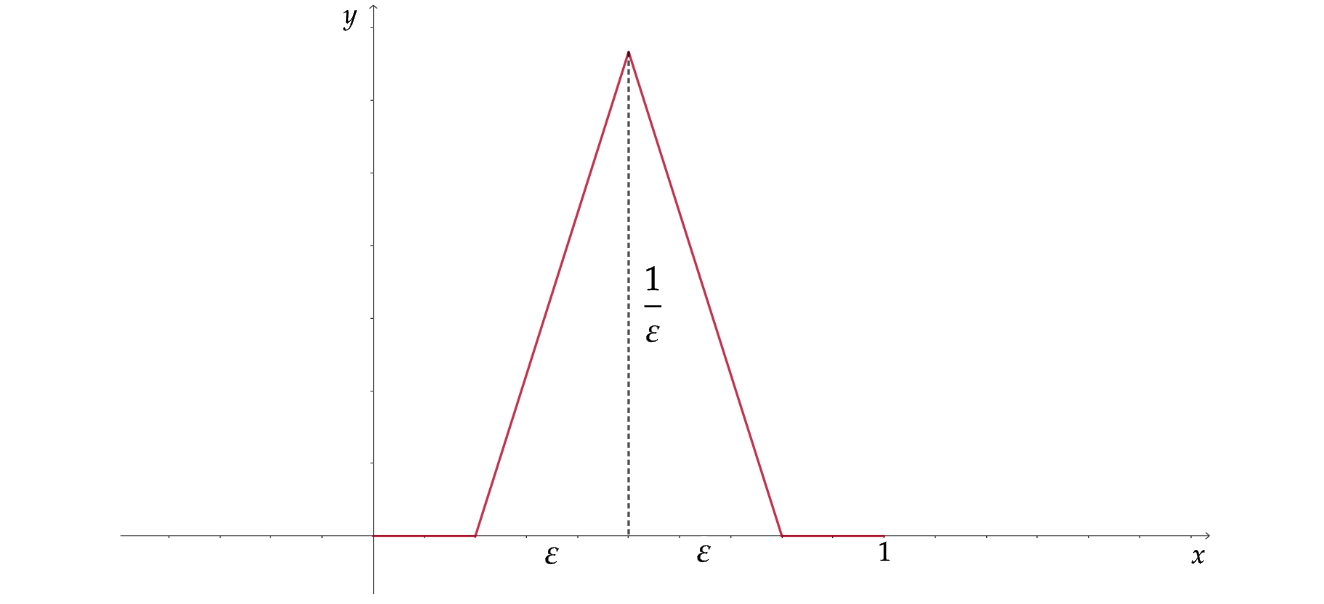
\includegraphics[scale=0.3]{Chapters/funcional1.png}\\
    \caption{Gráfica de $f_\varepsilon(x)$. Elaboración propia.}
    \end{figure}
    y sea
    \begin{align*}
        T:(C([0,1],\norm{\cdot}_1)&\longrightarrow (C([0,1]),\norm{\cdot}_\infty)\\
        f &\longmapsto Tf=f.
    \end{align*}
    Claramente $T$ es lineal al ser la aplicación identidad, veamos que
    \begin{align*}
        \norm{T}=\sup_{\substack{f\in C([0,1])\\||f||_1= 1}}\norm{Tf}_\infty=\sup_{\substack{f\in C([0,1])\\||f||_1= 1}}\norm{f}_\infty=\infty.
    \end{align*}
    Note que 
    \begin{align*}
        \norm{f_\varepsilon}_1&=\int_0^1 |f_\varepsilon(x)|\, dx\\
        &=\int_{\frac{1}{2}-\varepsilon}^{\frac{1}{2}}\left[\frac{1}{\varepsilon^2}\left(x-\frac{1}{2}\right)+\frac{1}{\varepsilon}\right]\, dx+\int_{\frac{1}{2}}^{\frac{1}{2}+\varepsilon}\left[-\frac{1}{\varepsilon^2}\left(x-\frac{1}{2}\right)+\frac{1}{\varepsilon}\right]\, dx\\
        &=\left[\frac{1}{\varepsilon^2}\left(\frac{x^2}{2}-\frac{x}{2}\right)+\frac{x}{\varepsilon}\right]\bigg|_{\frac{1}{2}-\varepsilon}^{\frac{1}{2}}+\left[-\frac{1}{\varepsilon^2}\left(\frac{x^2}{2}-\frac{x}{2}\right)+\frac{x}{\varepsilon}\right]\bigg|_{\frac{1}{2}}^{\frac{1}{2}+\varepsilon}\\
        &=\frac{1}{2}+\frac{1}{2}\\
        &=1,
    \end{align*}
    y
    \begin{align*}
        \norm{f_\varepsilon}_\infty=f_\varepsilon\left(\frac{1}{2}\right)=\frac{1}{\varepsilon},
    \end{align*}
    de esta manera
    \begin{align*}
        \norm{T}=\sup_{\substack{f\in C([0,1])\\||f||_1= 1}}\norm{f}_\infty\geq \norm{f_\varepsilon}_\infty=\frac{1}{\varepsilon},
    \end{align*}
    para todo $\varepsilon\in \left(0,\dfrac{1}{2}\right]$, por tanto
    \begin{align*}
        \norm{T}=\infty,
    \end{align*}
    concluyendo que $T$ no es continuo.
    \end{enumerate}
\end{proof}




%%%%%%%%%%%%%%%%%%%%%%%%%%

\textbf{Ejercicio 8:} Considere $E=c_0$ donde
$$c_0 =\{ u = \{u_n\}_{n\geq 1}: \text{ tales que } u_n\in \mathbb{R}, n\geq 1, \displaystyle\lim_{n\to\infty}u_n=0\}.$$
Es decir, $c_0$ es el conjunto de las secuencias reales que tienden a cero. Dotamos a este espacio con la norma $||u||_{\ell^{\infty}}=\displaystyle\sup_{n\in\mathbb{Z}^+}|u_n|$. Considere el funcional $f:E\to \mathbb{R}$ dado por 
$$f(u) = \displaystyle\sum_{n=1}^{\infty}\frac{1}{2^n}u_n.$$
\begin{itemize}
    \item[(i)] Muestre que $f\in E^*$ y calcule $||f||_{E^*}$.
    \item[(ii)] Es posible encontrar $u\in E$ tal que $||u||=1$ y $||f(u)=||f||_{E^*}$?
\end{itemize}

\begin{proof}
\begin{itemize}
    \item[(i)] Para ver que $f\in E^* = \mathcal{L}(E, \mathbb{R})$, debemos probar que el funcional $f$ es lineal y acotado.
    \begin{itemize}
        \item \textbf{Linealidad:}\\
        Sean $u = \{u_n\}, v = \{v_n\} \in c_0$, y $\alpha \in \mathbb{R}$. Note que $u+v \in c_0$ y $\alpha u \in c_0$. Así,
        \begin{align*}
            f(u + v) &= \sum_{n=1}^\infty \frac{1}{2^n} (u_n + v_n)\\
            &= \sum_{n=1}^\infty \left( \frac{1}{2^n} u_n + \frac{1}{2^n} v_n \right)\\
            &= f(u) + f(v),
        \end{align*}
        y, 
        \begin{align*}
            f(\alpha u) &= \sum_{n=1}^\infty \frac{1}{2^n} (\alpha u_n)\\
            &= \alpha \sum_{n=1}^\infty \frac{1}{2^n} u_n\\
            &= \alpha f(u).
        \end{align*}
        Luego, $f$ es lineal.

        \item \textbf{Acotado:}\\
        Sea $u \in c_0$, tiene que
        \begin{align*}
            |f(u)| &= \left| \sum_{n=1}^\infty \frac{1}{2^n} u_n \right|\\
            &\leq \sum_{n=1}^\infty \frac{1}{2^n} |u_n|\\
            &\leq \sum_{n=1}^\infty \frac{1}{2^n} \displaystyle\sup_{n\in\mathbb{Z}^+}|u_n|\\
            &\leq \sum_{n=1}^\infty \frac{1}{2^n} \|u\|\\
            &\leq \|u\|  \sum_{n=1}^\infty \frac{1}{2^n}\\
            &= \|u\| \left(2 - \dfrac{1}{2^0}\right)\\
            &= \|u\|.
        \end{align*}
        Luego $f$ es acotado.
    \end{itemize}
    De lo anterior se sigue que $f$ es lineal y acotado, es decir, $f\in E^*$.\\
    Ahora bien, como $|u_n|\leq \norm{u}\leq 1$, entonces
    $$|f(u)| \leq \norm{u}\leq 1.$$
    Así
    $$\|f\|_{E^*} := \sup_{\|u\| \leq 1} |f(u)| \leq 1.$$
    
    Ahora definamos una sucesión que se acerque al supremo. Sea
    $$u^{(N)} := (\underbrace{1, 1, \dots, 1}_{N \text{ veces }1}, 0, 0, \dots) \in c_0, \quad \text{con }  N \in \mathbb{N}.$$
    Note que $\|u^{(N)}\| = 1$, y
    $$f(u^{(N)}) = \sum_{n=1}^N \frac{1}{2^n} = 1 - \frac{1}{2^N}.$$
    Luego $\lim_{N \to \infty} f(u^{(N)}) = 1.$ Así
    $$1\leq \lim_{N \to \infty} f(u^{(N)}) \leq \sup_{\|u\| \leq 1} |f(u)| = \norm{f}_{E^*}.$$
    Concluimos que
    \[
    \|f\|_{E^*} = 1.
    \]
    \item[(ii)] Razonemos por el absurdo.\\
    Supongamos que existe $u \in c_0$ tal que $\|u\| = 1$ y $f(u) = \norm{f}_{E^*}= 1$. Como
    $$f(u) = \sum_{n=1}^\infty \frac{1}{2^n} u_n,$$
    esto implicaría que $\displaystyle\sum_{n=1}^\infty \frac{1}{2^n} u_n = 1$, que es el valor máximo posible dado que $\displaystyle\sum_{n=1}^\infty \frac{1}{2^n} = 1$ y $|u_n| \leq \|u\| = 1$. Para que esta igualdad sea valida, es necesario que $u_n = 1$ para todo $n$, pues en otro caso se perdería valor en la suma. Pero, la sucesión $u = (1,1,1,\dots) \notin c_0$, ya que no tiende a cero.
    
    Ahora bien, toda sucesión $u \in c_0$ cumple que $\displaystyle\lim_{n \to \infty} u_n = 0$. Esto implica que existe $N \in \mathbb{N}$ tal que $|u_n| < \varepsilon$ para $n \geq N$, para cualquier $\varepsilon > 0$. En particular, a pesar de que se consideren valores cercanos a 1 en los primeros términos de la sucesión, los términos posteriores deben tender a cero, lo que implica que
    $$f(u) = \sum_{n=1}^\infty \frac{1}{2^n} u_n < \sum_{n=1}^\infty \frac{1}{2^n} = 1.$$
    Por tanto, ningún elemento $u \in c_0$ satisface que $f(u) = 1$.
\end{itemize}
\end{proof}